\chapter{Arryas an Pointers}
In this chapter we are going to study about two very powerful constructs of C
programming; arrays and pointers. Arrays are what they are; array of some data
type. There can be an array of any complete type. You cannot create an array of
any incomplete type, therefore, an array of type void is not allowed. There are
fixed arrays and also variable length arrays. C99 inroduced variable length
arrays before that arrays were only of fixed length. However, you can increase
the capacity of a fixed sized array(not really array but a pointer) using
\texttt{realloc()} function. There is 
single-dimensional array and then there is multi-dimensional array. We will
first go through single-dimensional array then multi-dimensional.

\section{Single-Dimensional Array}
Let us first create a basic array and then see how to access it elements:

\begin{minted}[frame=single]{c}
#include <stdio.h>

int main()
{
  const int MAX = 8;
  //An initialized array to 0
  int a[8] = {0};
  //An uninitialized array
  int b[MAX];

  for(int i=0; i<8; i++)
  {
    b[i] = i;
    printf("b[%d]=%d\n", i, b[i]);
  }

  for(int i=0; i<8; i++)
  {
    printf("a[%d]=%d\n", i, a[i]);
  }

  return 0;
}
\end{minted}
and the output is:
\\\\\texttt{b[0]=0\\
b[1]=1\\
b[2]=2\\
b[3]=3\\
b[4]=4\\
b[5]=5\\
b[6]=6\\
b[7]=7\\
a[0]=0\\
a[1]=0\\
a[2]=0\\
a[3]=0\\
a[4]=0\\
a[5]=0\\
a[6]=0\\
a[7]=0\\\\}
Here you see array subscripting operator([ ]) in action. I have not covered this
particular operator in fourth chapter so it becomes my duty to explain it
here. There are two parts here one outside subscript and another outside. The
expression which is outside will have type “const pointer to object type”. This
means that array’s base address is fixed and cannot be changes. The expression
which is inside will have integer type. The result of these two has type
``type''. We will see pointer arithmetic with binary + operator in the pointers
section which is equivalent to subscript expression.

As you can see array a is fixed length array while array \texttt{b} is a
variable length array. You are not allowed to initialize variable length arrays
at the time of declaration. Notice that array indices do not start from 1 but
0. Never ever make the mistake of thinking that array indices start from 1. You
can also initialize an array as \texttt{a[]={1, 2, 3};} or \texttt{a[3]={1, 2,
    3};}. The array elements would be \texttt{a[0], a[1]} and \texttt{a[2]} in
both the cases. Notice how assignment is done to elements of second array
inside for loop one by one using the bracket operator or subscripting
operator. The array elements are always in sequence in memory. A conceptual
diagram is given below for first three elements of above array. Here 1 is the
value of first element.

\begin{figure}[H]
\begin{center}
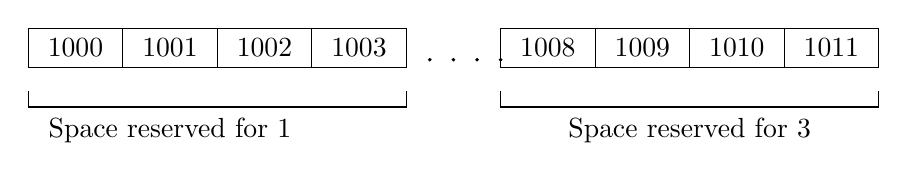
\begin{tikzpicture}
  \foreach \x in {0, ..., 3}
  \draw (\x*1.2cm, 0) -- +(1.2cm, 0) -- +(1.2cm, 0.5cm) -- +(0, .5cm) --
  cycle;
  \node at(5.1cm, .1cm) [circle,fill,inner sep=.5pt](a){};
  \node at(5.4cm, .1cm) [circle,fill,inner sep=.5pt](a){};
  \node at(5.7cm, .1cm) [circle,fill,inner sep=.5pt](a){};
  \node at(6cm, .1cm) [circle,fill,inner sep=.5pt](a){};
  \foreach \x in {0, ..., 3}
  \draw (\x*1.2cm+6cm, 0) -- +(1.2cm, 0) -- +(1.2cm, 0.5cm) -- +(0, .5cm) --
  cycle;
  \foreach \x [evaluate=\x as \xeval using \x+1000] in {0, ..., 3}
  \node at(\x*1.2cm + .6cm, .25cm) {\pgfmathtruncatemacro{\yet}{\xeval}\yet};
  \foreach \x [evaluate=\x as \xeval using \x+1008] in {0, ..., 3}
  \node at(\x*1.2cm+6.6cm, .25cm) {\pgfmathtruncatemacro{\yet}{\xeval}\yet};

  \draw (0, -.3cm) -- (0, -.5cm) -- (4.8cm, -.5cm) -- (4.8cm, -.3cm);
  \draw (6cm, -.3cm) -- (6cm, -.5cm) -- (10.8cm, -.5cm) -- (10.8cm, -.3cm);

  \node at (1.8cm, -.8cm) {Space reserved for 1};
  \node at (8.4cm, -.8cm) {Space reserved for 3};
\end{tikzpicture}
\caption{An Array's Memory Diagram}
\label{fig:An Array's Memory Diagram}
\end{center}
\end{figure}

Array elements are always(not always but most commonly. It is so common that I
have used always.) accessed using their indices so order of retrieval is $O(1)$
.(This is known as big-$O$ notation. You can find it in any Data Structure and
Algorithm book. The above program will not compile using old compilers which do
not support C99 standard like Turbo C++. Also, you may require to pass the flag
\texttt{-std=c99} or \texttt{-std=c11} to some versions of \texttt{gcc}. For
variable length arrays it is not necessary to declare the size in
advance. Even, input to program from other sources will do.

\begin{minted}[frame=single]{c}
#include <stdio.h>

int main()
{
  int i=0;

  printf("Enter the value of i:\n");
  scanf("%d", &i);
  getchar();
  char c[i];

  printf("Enter a string which contains one less no. of chars than i:\n");
  gets(c);
  puts(c);

  return 0;
}
\end{minted}
and the output is:
\\\\\texttt{Enter the value of i:\\
6\\
Enter a string which contains one less no. of chars than i:\\
shiv\\
shiv\\\\}
As you can see variable length array should be declared after the size is known
otherwise you may see strange output even though it is not compilation
error. For example you could have declaraed array immediately after \texttt{i}
but you will get some garbage output. The reason for this is that at that point
of time \texttt{i} contains garbage value. Also, note that array indices are
integers. Floating-point numbers or variables cannot be indices.

Now the question is why variable length arrays cannot initialized. If the size
of array is known at compile time then array can be initialized. The problem
with variable length array is that the variable's value may be in program or
come from user input. If it comes from user input then there is no way for
compiler to know that at compile time. Thus, to maintain consistency variable
length arrays are not initialized even if that variable has been assigned to in
the code.

Let us say you are writing a big piece of code and array is declared somewhere
and you want to know how many elemnets you can fill in the array or what is the
maximum size of array then you can use the following program:

\begin{minted}[frame=single]{c}

#include <stdio.h>

int main()
{
  float f[10]={0.0};

  printf("Size of array f is %zu.\n", sizeof(f)/sizeof(float));

  return 0;
}
\end{minted}
xand the output is:
\\\\\texttt{Size of array f is 10.\\\\}
Now an experienced programmer may ask that if we can know the size of array
then why we do not have something like out of bounds exception(i.e. accessing
elements having position beyong the size of array) of Java in C. My
answer to that is C was written in 1970 and Java in 1990. For example, there
are certain compilers with flags which help you detect this at runtime. You can
use \texttt{-fsanitize=address} which will help you detect the out of bounds
exception.

There are various ways in which you can define character arrays. For example,
\texttt{char c[6]={'h', 'e', 'l', 'l', 'o', '\textbackslash 0'};}. Remember, you must
terminate a character array with a null terminator. Another way to define the
same is: \texttt{char str[6] = "hello";}. In this example you do not need to
add \texttt{'\textbackslash 0'} explicitly as it is added automatically. Also, 6 is optional
here if you want you can ommit that. Of course second example is more
preferable. Note that if you declare an array of size \texttt{m} and data type
size of array is \texttt{n} bytes then the array will consume \texttt{m*n}
bytes no matter what; even when you are not using those bytes. Note that all
these arrays are on stack memory area. We will see how to allocate array(in
form of pointers) on heap memory area once we have studied pointers.

\section{Multi-Dimensional Arrays}
Arrays can be n-dmensional. There is no limit on dimensions. You can allocate
as much as your memory allows. We will begin with two-dimensional array. A
two-dimensional array looks like a matrix. Say a two-dimensional array has
\texttt{m} as one dimension and \texttt{n} as second diemnsion. Then total
no. of elements will be \texttt{m*n} and size occupied is \texttt{m*n*size of
  data type} of array. There are various ways to initialize a two-dimensional
array. Consider the following example:

\begin{minted}[frame=single]{c}
#include <stdio.h>

int main()
{
  int a[2][2] = {{1,2},{3,4}};
  int b[2][2] = {1,2,3,4};

  //iterating over array
  for(int i=0;i<2;i++)
  {
    for(int j=0;j<2;j++)
      printf("%d ", a[i][j]);
    printf("\n");
  }
  for(int i=0;i<2;i++)
  {
    for(int j=0;j<2;j++)
      printf("%d ", b[i][j]);
    printf("\n");
  }

  return 0;
}
\end{minted}
and the output is:
\\\\\texttt{1 2\\
3 4\\
1 2\\
3 4\\\\}
Thus, you see that allocation is first for latter dimension. Same holds trur
for more than 2 dimensions. Typical usage of two dimensional arrays is in
representation of structures which have a matrix representation, array of
strings, system of linear equations etc. For example, a csv file can be
represented by a two dimensional matrix.

Same way you can have multi-dimensional array. I leave it up to you to find
applications of different arrays. For now, try multiplying two matrices, doing
a transpose, inverse of a matrix and printing a yearly calenday for any year
for example. With the current information given to you, you should be able to
do all these easily. As shown for array a it is not really a single array but
an array of array. How we can read this is array a has two arrays each of which
have two integers.

\section{Pointers}
A pointer can store an address. A pointer of some type can store address of
that type and a pointer to void can store address of any type. Pointers are
possibly most powerful construct among all. Pointers are very much similar like
arrays in the sense that they also require contguous memory locations to be
available for allocation. Also, pointers can also be accessed like arrays using
subscript([ ]) operator.

There are four standard library functions associated with them. All these are
declared in \texttt{stdlib.h} which is part of standard c library. The
functions are: \texttt{malloc(), calloc(), realloc()} and
\texttt{free()}. Following is the contents of man pages verbatim,later in the
program you can go to opengroup links as well. Given below are signatures of
these functions:

\begin{minted}[frame=single]{c}
void *calloc(size_t nmemb, size_t size);
void *malloc(size_t size);
void free(void *ptr);
void *realloc(void *ptr, size_t size);
\end{minted}

here \texttt{size\_t} is the unsigned integer type of the result of the
\texttt{sizeof} operator. It is defined in \texttt{stddef.h}.
Descriptions from man page are given below:

\texttt{calloc()} allocates memory for an array of nmemb elements of
\texttt{size} bytes each and returns a pointer to the allocated memory. The
memory is set to zero. If \texttt{nmemb} or size is 0, then \texttt{calloc()}
returns either \texttt{NULL}, or a unique pointer value that can later be
successfully passed to \texttt{free()}.

\texttt{malloc()} allocates \texttt{size} bytes and returns a pointer to the
allocated memory. The memory is not cleared. If \texttt{size} is 0, then
\texttt{malloc()} returns either \texttt{NULL}, or a unique pointer value that
can later be successfully passed to \texttt{free()}.

\texttt{free()} frees the memory space pointed to by \texttt{ptr}, which must
have been returned by a previous call to \texttt{malloc(), calloc()} or
\texttt{realloc()}. Otherwise, or if \texttt{free(ptr)} has already been called
before, undefined behavior occurs. If \texttt{ptr} is \texttt{NULL}, no
operation is performed.

\texttt{realloc()} changes the size of the memory block pointed to by
\texttt{ptr} to \texttt{size} bytes. The contents will be unchanged to the
minimum of the old and new sizes; newly allocated memory will be
uninitialized. If \texttt{ptr} is \texttt{NULL}, then the call is equivalent to
\texttt{malloc(size)}, for all values of \texttt{size}; if \texttt{size} is
equal to zero, and \texttt{ptr} is not \texttt{NULL}, then the call is
equivalent to \texttt{free(ptr)}. Unless \texttt{ptr} is \texttt{NULL}, it must
have been returned by an earlier call to \texttt{malloc(), calloc()} or
\texttt{realloc()}. If the area pointed to was moved, a \texttt{free(ptr)} is
done.

Let us consider a program:

\begin{minted}[frame=single]{c}
#include <stdio.h>
#include <stdlib.h>

int main()
{
  int *p = NULL;

  p = (int*)malloc(sizeof(int)*8);

  for(int i=0;i<8;i++)
  {
    *(p+i)=i;
    printf("Content at %dth location is %d.\n", i, *(p+i));
  }

  return 0;
}
\end{minted}
and the output is:
\\\\\texttt{Content at 0th location is 0.\\
Content at 1th location is 1.\\
Content at 2th location is 2.\\
Content at 3th location is 3.\\
Content at 4th location is 4.\\
Content at 5th location is 5.\\
Content at 6th location is 6.\\
Content at 7th location is 7.\\\\}
We could have written the same program in a different way using subscript
operator as shown below:

\begin{minted}[frame=single]{c}
#include <stdio.h>
#include <stdlib.h>

int main()
{
  int *p = NULL;

  p = (int*)malloc(sizeof(int)*8);

  for(int i=0;i<8;i++)
  {
    p[i]=i;
    printf("Content at %dth location is %d.\n", i, p[i]);
  }

  return 0;
}
\end{minted}

A postfix expression followed by an expression in square brackets \texttt{[]}
is a subscripted designation of an element of an array object. The definition
of the subscript operator \texttt{[]} is that \texttt{E1[E2]} is identical to
\texttt{(*((E1)+(E2)))}. Because of the conversion rules that apply to the
binary \texttt{+} operator, if \texttt{E1} is an array object (equivalently, a
pointer to the initial element of an array object) and \texttt{E2} is an
integer, \texttt{E1[E2]} designates the \texttt{E2}-th element of \texttt{E1}
(counting from zero).

\subsection{Pointer Arithmetic}
Addition and subtarction of pointers was not covered in the chapter of
operators and 
expressions. When an expression that has integer type is added to or subtracted
from a pointer, the result has the type of the pointer operand. If the pointer
operand points to an element of an array object, and the array is large enough,
the result points to an element offset from the original element such that the
difference of the subscripts of the resulting and original array elements
equals the integer expression. In other words, if the expression \texttt{P}
points to the \texttt{i}-th element of an array object, the expressions
\texttt{(P)+N} (equivalently, \texttt{N+(P)}) and \texttt{(P)-N} (where
\texttt{N} has the value \texttt{n}) point to, respectively, the
\texttt{i+n}-th and \texttt{i-n}-th elements of the array object, provided they
exist. Moreover, if the expression \texttt{P} points to the last element of an
array object, the expression \texttt{(P)+1} points one past the last element of
the array object, and if the expression \texttt{Q} points one past the last
element of an array object, the expression \texttt{(Q)-1} points to the last
element of the array object. If both the pointer operand and the result point
to elements of the same array object, or one past the last element of the array
object, the evaluation will not produce an overflow; otherwise, the behavior is
undefined. If the result points one past the last element of the array object,
it will not be used as the operand of a unary \texttt{*} operator that is
evaluated.

When two pointers are subtracted, both shall point to elements of the same
array object, or one past the last element of the array object; the result is
the difference of the subscripts of the two array elements. The size of the
result is implementation-defined, and its type (a signed integer type) is
\texttt{ptrdiff\_t} defined in the \texttt{\textless stddef.h\textgreater}
header. If the result is not representable in an object of that type, the
behavior is undefined. In other words, if the expressions \texttt{P} and
\texttt{Q} point to, respectively, the \texttt{i}-th and \texttt{j}-th elements
of an array object, the expression \texttt{(P)-(Q)} has the value \texttt{i-j}
provided the value fits in an object of type \texttt{ptrdiff\_t}. Moreover, if
the expression \texttt{P} points either to an element of an array object or one
past the last element of an array object, and the expression \texttt{Q} points
to the last element of the same array object, the expression
\texttt{((Q)+1)-(P)} has the same value as \texttt{((Q)-(P))+1} and as
\texttt{-((P)-((Q)+1))}, and has the value zero if the expression \texttt{P}
points one past the last element of the array object, even though the
expression \texttt{(Q)+1} does not point to an element of the array object.

An example is given below:

\begin{minted}[frame=single]{c}
#include <stdio.h>
#include <stdlib.h>

int main()
{
  int *p = (int*)malloc(sizeof(int)*2);
  p[0] = 1;
  p[1] = 2;

  printf("%p %p\n", &p[0], &p[1]);
  printf("%td %td\n", &(p[0]) - &(p[1]), &(p[1]) - &p[0]);
  free(p);

  return 0;
}
\end{minted}
and the output is:
\\\\\texttt{0x7f8b5b404b10 0x7f8b5b404b14\\
-1 1\\\\}
As you can see the absolute values of addresses differ by 4 but when converted
to difference it is divided by size of data type or is given by differebce in
position.

You can also apply increment and decrement operators on pointers. I will show
you a reimplementation of previos program using increment operator:

\begin{minted}[frame=single]{c}
#include <stdio.h>
#include <stdlib.h>

int main()
{
  int *p = NULL;

  p = (int*)malloc(sizeof(int)*8);
  int *q = p;

  for(int i=0;i<8;i++)
  {
    *(p+i)=i;
    printf("Content at %dth location is %d.\n", i, *(q++));
  }

  return 0;
}
\end{minted}
and the output is:
\\\\\texttt{Content at 0th location is 0.\\
Content at 1th location is 1.\\
Content at 2th location is 2.\\
Content at 3th location is 3.\\
Content at 4th location is 4.\\
Content at 5th location is 5.\\
Content at 6th location is 6.\\
Content at 7th location is 7.\\\\}

\section{Address-of and Indirection Operators}
As is the case with subscript operator and pointer arithmetic in the fourth
chapter that I have delayed these two as well for I wanted to put them
here. Whenever you declare a plain variable you have an address associated with
it and that variable is an lvalue. Just to repeat an lvalue is a value whose
address can be taken. To take the address of an lvalue you use the address
operator which is \texttt{\&}. Now a pointer points to address of any value as
we know so we can use address operator to get the address and use a pointer to
store. There are several usage of storing an address. Most notable of those is
pass-by-address which we will see in next chapter which will deal with
functions. Let us say we take address of a variable and assign that to a
pointer. Then if we change the value of the memory pointed to by the pointer
then the variable whose address has been taken will get updated with this new
value. Consider for example:

\begin{minted}[frame=single]{c}
#include <stdio.h>

int main()
{
  int  i = 8;
  int *p = &i;

  *p = 7;

  printf("i=%d *p=%d\n", i, *p);

  return 0;
}
\end{minted}
and the output is:
\\\\\texttt{i=7 *p=7\\\\}
Note that since both \texttt{i} and \texttt{p} are sharing address as
\texttt{p} is assigned the address of \texttt{i} changing the value of one will
have effect on the other. For exmaple:

\begin{minted}[frame=single]{c}
#include <stdio.h>

int main()
{
  int  i = 8;
  int *p = &i;

  *p = 7;

  printf("i=%d *p=%d\n", i, *p);

  *p = 10;

  printf("i=%d *p=%d\n", i, *p);

  return 0;
}
\end{minted}
and the output is:
\\\\\texttt{i=7 *p=7\\
i=10 *p=10\\\\}
So you see the power of pointers that if you have an address you can modify its
contents. This is exacly what \texttt{scanf()} does. The dereference operator
or indirection operator or asterisk (\texttt{*}) gives you value at address
pointed to by pointer o. However, if you want to change address of some varible
like that ofi by doing something like \texttt{\&i=\&someOthervar;} you cannot do that
because address is not an lvalue. However, you can pass address of a pointer
variable to some other function and use it using pointer to pointer notation
which I will show you in next chapter. As I have shown pointers are kind of
equivalent to array except the fact that they are on heap and sizeof operator
will not work on them. Consider this example:

\begin{minted}[frame=single]{c}
#include <stdio.h>
#include <stdlib.h>

int main()
{
  int  a[4] = {1,2,3,4};
  int* p    = a;
  int* q    = (int*)calloc(10, 4);

  for(int i=0; i<4; i++)
    printf("i=%d *p=%d\n", i, *(p+i));

  printf("Size of a=%d\n", sizeof(a));
  printf("Size of p=%d\n", sizeof(p));
  printf("Size of q=%d\n", sizeof(q));

  return 0;
}
\end{minted}
and the output is:
\\\\\texttt{i=0 *p=1\\
i=1 *p=2\\
i=2 *p=3\\
i=3 *p=4\\
Size of a=16\\
Size of p=4\\
Size of q=4\\\\}
Here \texttt{p} acts as pointer to array. You can have a pointer to any kind of
array. You can point to any element of array because array elements are lvalues
whose addresses can be taken and to initialize a pointer alll you need is an
address.

Complex pointer arithmetic is best avoided. Be very thoughtful that if you
really really need it. Use loops to iterate arrays. Multiple levels of
indirection is also bad. Typically I have not seen more than pointers to
pointers. Now we will see array of pointers.

\section{Arrays of Pointers}
Pointers are like ordinary variables in many ways, so we can as well create
array of pointers. Consider following for example:

\begin{minted}[frame=single]{c}
#include <stdio.h>
#include <stdlib.h>

int main()
{
  char* strArray[2]={"Hello", "Universe!"};

  for(int i=0; i<2; i++)
    printf("%s\n", strArray[i]);

  return 0;
}
\end{minted}
and the output is:
\\\\\texttt{Hello\\
Universe!\\\\}
Note how the length of two array elements are different as they are
pointers. Let us do a more complex example:

\begin{minted}[frame=single]{c}
#include <stdio.h>
#include <stdlib.h>

int main()
{
  int* intArray[2];

  intArray[0] = (int*)calloc(3, sizeof(int));
  intArray[1] = (int*)calloc(2, sizeof(int));

  *intArray[0]     = 4;
  *(intArray[0]+1) = 5;
  *(intArray[0]+2) = 6;


  *intArray[1]     = 1;
  *(intArray[1]+1) = 2;

  for(int i=0; i<3; i++)
  {
    printf("Memory location=%p Content=%d\n", intArray[0]+i, *(intArray[0]+i));
  }

  for(int i=0; i<2; i++)
  {
    printf("Memory location=%p Content=%d\n", intArray[1]+i, *(intArray[1]+i));
  }

  return 0;
}
\end{minted}
and the output is:
\\\\\texttt{Memory location=0x87d1008 Content=4\\
Memory location=0x87d100c Content=5\\
Memory location=0x87d1010 Content=6\\
Memory location=0x87d1018 Content=1\\
Memory location=0x87d101c Content=2\\\\\\}
Note missing four bytes between 6 and 1. Memory locations may be different on
your system. But see how messy pointer syntax can go even with such simple
code. Array to pointers are useful for containing variables of dynamic size of
same type.

\section{Pointers of Pointers}
Pointers to pointers are same as array of pointers. The only difference is that
you can dynamically modify the number of elements. Consider the following
example:

\begin{minted}[frame=single]{c}
#include <stdio.h>
#include <stdlib.h>

int main()
{
  int** intPtr;

  intPtr = (int**)malloc(sizeof(sizeof(int*)*2));

  *intPtr = (int*)malloc(sizeof(int)*3);
  *(intPtr+1) = (int*)malloc(sizeof(int)*4);

  **intPtr     = 1;
  *(*intPtr+1) = 2;
  *(*intPtr+2) = 7;


  **(intPtr+1)      = 3;
  *(*(intPtr+1)+1)  = 5;
  *(*(intPtr+1)+2)  = 9;
  *(*(intPtr+1)+3)  = 11;

  for(int i=0; i<3; i++)
    printf("Memory location=%p content=%d\n", *intPtr+i, *(*intPtr+i));

  for(int i=0; i<4; i++)
    printf("Memory location=%p content=%d\n", *(intPtr+1)+i, *(*(intPtr+1)+i));

  return 0;
}
\end{minted}
and the output is:
\\\\\texttt{Memory location=0x9947018 content=1\\
Memory location=0x994701c content=2\\
Memory location=0x9947020 content=7\\
Memory location=0x9947028 content=3\\
Memory location=0x994702c content=5\\
Memory location=0x9947030 content=9\\
Memory location=0x9947034 content=11\\\\}
Again memory location may change on your system. As you can see how things can
get messy with pointers. Believe me you will hate this. Also, I do not see any
reason to use more than two levels of indirection. So you get the idea. If you
need dynamic no. of elements with dynamic content you are going to use pointers
to pointers.

\section{\texttt{realloc()} Function}
Once \texttt{malloc()} and \texttt{calloc()} allocate some memory you have that
certain amount of memory available to you. When you have an array you have some
memory but what if you want more later. \texttt{reallloc()} comes to rescue
you. Here is a sample program:

\begin{minted}[frame=single]{c}
#include <stdio.h>
#include <stdlib.h>

int main()
{
  int *p = (int*)malloc(sizeof(int)*2);

  *p     = 5;
  *(p+1) = 7;

  printf("Original 1st element=%d\n", *p);
  printf("Original 2nd element=%d\n", *(p+1));

  p = (int*)realloc(p, sizeof(int)*4);

  *(p+2) = 9;
  *(p+3) = 11;

  printf("New 1st element=%d\n", *p);
  printf("New 2nd element=%d\n", *(p+1));
  printf("New 3rd element=%d\n", *(p+2));
  printf("New 4th element=%d\n", *(p+3));

  return 0;
}
\end{minted}
and the output is:
\\\\\texttt{Original 1st element=5\\
Original 2nd element=7\\
New 1st element=5\\
New 2nd element=7\\
New 3rd element=9\\
New 4th element=11\\\\}

\section{\texttt{free} Function}
Whatever program we have written in this chapter related to dynamic memory
allocation using malloc() etc are bad code just because we are not releasing
memory properly. Any call to memory allocation functions have to be matched
with a corresponding free() call. The reason for this is that when all pointers
to a memory area are lost and that memory is not freed then operating system
cannot recycle that memory. In case of servers or long running processes this
may eat up all the physical RAM and virtual memory and eventually freeze the
system. To guard against such events you must macth all allocation calls with
deallocation calls so that operating system can reclaim the freed memmory.

You must heed this warning given here with all of your focus. You got to handle
heap that is dynamically allocated memory yourself. You allocate and you free
it. If you miss you have a memory leak.

\section{Constness of Pointers}
To make anything constant you need to associate const keyword with it. For
example, \texttt{const int i; const float f;}. However, with pointers in
picture scenarios change compared to two simple previous examples. When
pointers are made constant there are two elements. First is the pointer itself
and second is the value pointed to. Consider for example:

\begin{minted}[frame=single]{c}
const int* i;  //constant pointer data is not
int* const i;  //constant data pointer is not
const int* const i; //both are const
\end{minted}
The way to read it is you draw a vertical line where asterisk(\texttt{*}) is
there and the value associated with const is constant. Whenever you need use a
constant freely. Try to use constants more and more. Also, prefre them to
following:

\begin{minted}[frame=single]{c}
#define MAX 10
\end{minted}

It will replace \texttt{MAX} with 10 in the file everywhere without any concern
of type-safety. Also, it does not enter in the symbol table so while debugging
you will not see \texttt{MAX} anywhere. So instead you should use something
like:

\begin{minted}[frame=single]{c}
const int MAX=10;
\end{minted}

I will also like to say something about volatile variables. Beginners are
usually convinced that volatile variables cannot be declraed as const. Let me
iterate the definitions once again. A const variable cannot be modifed by the
program itself. A volatile variable can be modified by sources other than the
program itself. Hence, a const volatile variable cannot be modified by the
program but other sources can still modify it.
